\begin{name}
	{\tenchude}
	{\tendethi}
	{\tentruong}
	{\thoigian}
\end{name}
\TN
\Opensolutionfile{ans}[ans/ans\currfilebase]
%% -- Câu 1 --%%
\begin{ex}%%[Dự án đề kiểm tra Toán 12 GHKI NH25-26- Nguyễn Văn Sang ]%[THPT NGUYỄN BỈNH KHIÊM - Hà Nội]%[2D1N1-2]
	Cho hàm số $y=f(x)$ có bảng biến thiên như hình vẽ sau.
	\begin{center}
		
\begin{tikzpicture}[scale=1, font=\footnotesize, line join=round, line cap=round, >=stealth]
			\tkzTabInit[nocadre=false,lgt=1,espcl=2,deltacl=0.5]
			{$x$/1, $f'(x)$/1, $f(x)$/2}
			{$-\infty$, $-1$, $3$, $+\infty$}
			\tkzTabLine{, - ,  0 ,  + ,  0 ,  - ,}
			\tkzTabVar{+/$+\infty$ , -/$0$ , +/$4$ , -/$-\infty$}
		\end{tikzpicture}
	\end{center}
	Hàm số đã cho đồng biến trên khoảng nào sau đây?
	\choice
	{ $(0;4)$ }
	{\True $(-1;3)$ }
	{ $(0;+\infty)$ }
	{ $(-\infty;4)$ }
	\loigiai{
		Từ bảng dấu đạo hàm ta có $f'(x)>0$ trên khoảng $(-1,3)$, nên hàm số đã cho đồng biến trên khoảng $(-1,3)$.
	}
\end{ex}
%% -- Câu 2 --%%
\begin{ex}%%[Dự án đề kiểm tra Toán 12 GHKI NH25-26- Nguyễn Văn Sang ]%[THPT NGUYỄN BỈNH KHIÊM - Hà Nội]%[2D1N2-2]
	\immini[thm]{Cho hàm số $y=f(x)$ có đồ thị như hình vẽ bên. Hàm số đã cho đạt cực đại tại điểm nào sau đây?
		\choice
		{$x=2$}
		{$x=-3$}
		{$x=1$}
		{\True $x=-1$}}{
		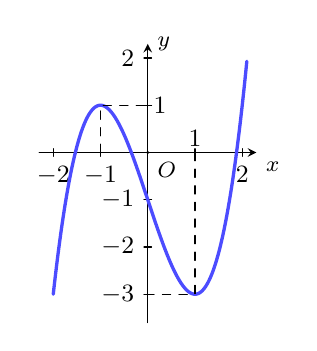
\begin{tikzpicture}[scale=.6, font=\footnotesize, line join=round, line cap=round, >=stealth]
			\def\xmin{-2.3} \def\xmax{2.3}
			\def\ymin{-3.6} \def\ymax{2.3}
			% Trục tọa độ
			\draw[->] (\xmin,0) -- (\xmax,0) node[below right] {$x$};
			\draw[->] (0,\ymin) -- (0,\ymax) node[right] {$y$};
			
			\foreach \x in {1}
			\draw (\x,0.08) -- (\x,-0.08) node[above] {\small $\x$};
			\foreach \x in {-2,-1,2}
			\draw (\x,0.08) -- (\x,-0.08) node[below] {\small $\x$};
			\foreach \y in {-3,-2,-1,2}
			\draw (0.08,\y) -- (-0.08,\y) node[left] {\small $\y$};
			\foreach \y in {1}
			\draw (0.08,\y) -- (-0.08,\y) node[right] {\small $\y$};
			\fill (0,0) circle (1pt) node[below right]{$O$};
			\draw[very thick, blue!70]
			plot[domain=-2:2.1, samples=300]
			({\x},{\x*\x*\x - 3*\x - 1});
			\draw[dashed] (-1,0) |- (0,1);
			\draw[dashed] (1,0) |- (0,-3);
		\end{tikzpicture}
	}
	\loigiai{
		Từ đồ thị, hàm số đạt cực đại tại $x=-1$.
	}
\end{ex}
%% -- Câu 3 --%%
\begin{ex}%%[Dự án đề kiểm tra Toán 12 GHKI NH25-26- Nguyễn Văn Sang ]%[THPT NGUYỄN BỈNH KHIÊM - Hà Nội]%[2D1N3-1]
	Lợi nhuận trước thuế theo quý của công ty X được cho bởi biểu đồ sau đây. Từ quý I năm $2021$ đến quý III năm $2022$, lợi nhuận trước thuế theo quý của công ty X đạt giá trị lớn nhất bằng bao nhiêu tỷ đồng?
	\begin{center}
		\begin{tikzpicture}[scale=.6, font=\footnotesize, line join=round, line cap=round, >=stealth, x=2.285714cm, y=0.0233333cm] % 16/7 cm, 7/300 cm
			% Miền vẽ
			\def\xmin{0} \def\xmax{7.5}
			\def\ymin{0}   \def\ymax{320}
			% Nhấn mạnh các vạch ngang chính (0,50,...,300)
			\foreach \Y in {0,50,100,150,200,250,300}{
				\draw[gray!40, line width=0.6pt] (\xmin,\Y) -- (\xmax,\Y);
			}
			
			% Trục tọa độ với mũi tên
			\draw[very thick, -stealth] (\xmin,0) -- (\xmax,0) node[below right] {Quý};
			\draw[very thick, -stealth] (0,\ymin) -- (0,\ymax) node[above right] {Tỷ đồng};
			
			% Ticks và nhãn trục X tại 1..7 với nhãn quý
			\foreach \X/\LAB in {
				1/{QI/21},
				2/{QII/21},
				3/{QIII/21},
				4/{QIV/21},
				5/{QI/22},
				6/{QII/22},
				7/{QIII/22}
			}{
				\draw (\X,0) -- (\X,-3); % vạch nhỏ dài 3 đơn vị y (~0.07 cm)
				\node[below] at (\X,0) {\LAB};
			}
			
			% Ticks và nhãn trục Y tại 0..300 cách 50
			\foreach \Y in {0,50,100,150,200,250,300}{
				\draw (0,\Y) -- (-0.05,\Y); % vạch nhỏ
				\node[left] at (0,\Y) {\Y};
			}
			% Dữ liệu các quý (đường gấp khúc)
			\draw[blue, very thick]
			(1,150) -- (2,185) -- (3,145) -- (4,205) -- (5,155) -- (6,270) -- (7,60);
			% Dấu chấm tại các điểm (mark=*)
			\foreach \X/\Y in {1/150,2/185,3/145,4/205,5/155,6/270,7/60}{
				\filldraw[blue, line width=1pt, fill=white] (\X,\Y) circle (3pt);
			}
			% Ghi số liệu bên cạnh các điểm (giống anchor mẫu)
			\node[blue] at (1,150) [anchor=south] {150};
			\node[blue] at (2,185) [anchor=south] {185};
			\node[blue] at (3,145) [anchor=north] {145};
			\node[blue] at (4,205) [anchor=south] {205};
			\node[blue] at (5,155) [anchor=north] {155};
			\node[blue] at (6,270) [anchor=south] {270};
			\node[blue] at (7,60)  [anchor=north] {60};
		\end{tikzpicture}
	\end{center}
	\choice
	{$270$}
	{$60$}
	{\True $205$}
	{$300$}
	\loigiai{
		Quan sát biểu đồ: các giá trị lần lượt là $150$, $185$, $145$, $205$, $155$, $270$, $60$.\\
		Giá trị lớn nhất trong các số này là $270$.\\
		Vậy lợi nhuận lớn nhất bằng $270$ tỷ đồng.
	}
\end{ex}
%% -- Câu 4 --%%
\begin{ex}%%[Dự án đề kiểm tra Toán 12 GHKI NH25-26- Nguyễn Văn Sang ]%[THPT NGUYỄN BỈNH KHIÊM - Hà Nội]%[2D1N4-1]
	Đồ thị hàm số $y=\dfrac{2x+1}{x-1}$ có đường tiệm cận đứng và tiệm cận ngang lần lượt là
	\choice
	{$x=2, y=1$}
	{\True $x=1, y=2$}
	{$x=-1, y=2$}
	{$x=1, y=-2$}
	\loigiai{
		Xét hàm số $y=\dfrac{2x+1}{x-1}$.\\
		Ta có $\displaystyle \lim_{x\to 1^\pm} \dfrac{2x+1}{x-1}=\pm\infty$ nên đường tiệm cận đứng là $x=1$.\\
		Ta ccó $\displaystyle \lim_{x\to\pm\infty} \dfrac{2x+1}{x-1}=2$ nên đường tiệm cận ngang là $y=2$.\\
		Vậy tiệm cận đứng $x=1$, tiệm cận ngang $y=2$.
	}
\end{ex}
%% -- Câu 5 --%%
\begin{ex}%%[Dự án đề kiểm tra Toán 12 GHKI NH25-26- Nguyễn Văn Sang ]%[THPT NGUYỄN BỈNH KHIÊM - Hà Nội]%[2D1N5-1]
	\immini
	{Đường cong trong hình vẽ bên là đồ thị của hàm số nào sau đây?
		\choice
		{\True $y=-x^3-3x^2+1$}
		{$y=-x^3+3x^2+1$}
		{$y=-x^3-3x+1$}
		{$y=-x^3+3x+1$}}
	{
		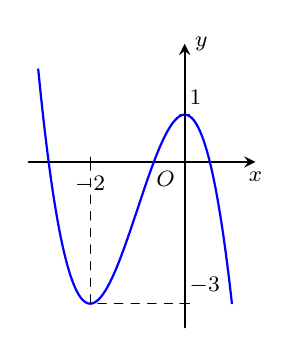
\begin{tikzpicture}[scale=.6, font=\footnotesize, line join=round, line cap=round, >=stealth]
			\draw[-stealth, thick] (-3.3,0) -- (1.5,0) node[below] {$x$};
			\draw[-stealth, thick] (0,-3.5) -- (0,2.5) node[right] {$y$};
			\node at (0,0) [below left] {$O$};
			\foreach \x in {-2}
			\draw (\x,0.1) -- (\x,-0.1) node[below] {$\x$};
			\foreach \y in {-3,1}
			\draw (0.1,\y) -- (-0.1,\y) node[above right] {$\y$};
			\draw[blue, thick, domain=-3.1:1, samples=200] 
			plot (\x, {-(\x)^3 - 3*(\x)^2 + 1});
			\draw[dashed] (-2,0) |- (0,-3);
			\draw[dashed] (0,1) -- (0,0);
		\end{tikzpicture}
	}
	\loigiai{
		Đồ thị đi qua điểm $(-2;-3)$.\\
		Thử với $y=-x^3-3x^2+1$ có $f(-2)=8-12+1=-3$ đúng với hình vẽ.\\
		Các phương án khác cho giá trị khác $-3$.\\
		Vậy chọn $y=-x^3-3x^2+1$.\\
	}
\end{ex}
%% -- Câu 6 --%%
\begin{ex}%%[Dự án đề kiểm tra Toán 12 GHKI NH25-26- Nguyễn Văn Sang ]%[THPT NGUYỄN BỈNH KHIÊM - Hà Nội]%[2D1N5-1]
	Bảng biến thiên dưới đây là của hàm số nào trong số các hàm số được cho trong các đáp án A, B, C, D?
	\begin{center}
		
\begin{tikzpicture}[scale=1, line join=round, line cap=round, >=stealth]
			\tkzTabInit[nocadre=false,lgt=1.5,espcl=2,deltacl=0.5]
			{$x$/1, $f'(x)$/1, $f(x)$/2}
			{$-\infty$, $1$, $+\infty$}
			\tkzTabLine{, + ,  d ,  + ,}
			\tkzTabVar{-/$2$ , +D-/$+\infty$/$-\infty$ , +/$2$}
		\end{tikzpicture}
	\end{center}
	\choice
	{\True $y=\dfrac{2x-3}{x-1}$}
	{$y=\dfrac{x-1}{x-2}$}
	{$y=\dfrac{2x-1}{x-1}$}
	{$y=\dfrac{2x+1}{x-1}$}
	\loigiai{
		Từ bảng biến thiên: hàm số có tiệm cận đứng $x=1$, tiệm cận ngang $y=2$ và $y'>0$ trên từng khoảng xác định.
		\begin{itemize}
			\item Với $y=\dfrac{2x-3}{x-1}$ có $y'=\dfrac{1}{(x-1)^2}>0$ (phù hợp).
			\item Với $y=\dfrac{2x-1}{x-1}$ có $y'=\dfrac{-1}{(x-1)^2}<0$ (nghịch biến, loại).
			\item Với $y=\dfrac{2x+1}{x-1}$ có $y'=\dfrac{-3}{(x-1)^2}<0$ (nghịch biến, loại).
		\end{itemize}
		Vậy chọn $y=\dfrac{2x-3}{x-1}$.
	}
\end{ex}
%% -- Câu 7 --%%
\begin{ex}%%[Dự án đề kiểm tra Toán 12 GHKI NH25-26- Nguyễn Văn Sang ]%[THPT NGUYỄN BỈNH KHIÊM - Hà Nội]%[2D1N2-1]
	Cho hàm số $y=f(x)$ xác định trên $\mathbb{R}$ và có đạo hàm $f'(x)=(x+2)(x^2-1)(x+1)$ với mọi số thực $x$. Giá trị cực tiểu của hàm số $y=f(x)$ bằng
	\choice
	{\True $f(1)$}
	{$f(-1)$}
	{$f(-2)$}
	{$f(0)$}
	\loigiai{
		Ta có $f'(x)=(x+2)(x^2-1)(x+1)=(x+2)(x-1)(x+1)^2$.\\
		Giải $f'(x)=0$ có
		$$
		(x+2)(x-1)(x+1)^2=0 \Leftrightarrow \hoac{&x=-2\\& x=-1\\& x=1.}
		$$
		Lập bảng xét dấu đạo hàm
		\begin{center}
			
\begin{tikzpicture}
				\tkzTabInit[lgt=2,espcl=2]
				{$x$/1,$f'(x)$/1}
				{$-\infty$,$-2$,$-1$,$1$,$+\infty$}
				\tkzTabLine{,+,0,-,0,-,0,+,}
			\end{tikzpicture}
		\end{center}
		Tại $x=1$, $f'(x)$ đổi dấu từ âm sang dương $\Rightarrow$ hàm số đạt cực tiểu tại $x=1$.\\
		Giá trị cực tiểu là $f(1)$.\\
	}
\end{ex}
%% -- Câu 8 --%%
\begin{ex}%%[Dự án đề kiểm tra Toán 12 GHKI NH25-26- Nguyễn Văn Sang ]%[THPT NGUYỄN BỈNH KHIÊM - Hà Nội]%[2D1N2-1]
	Cho hàm số $y=f(x)$ liên tục trên $\mathbb{R}$ và có bảng xét dấu của đạo hàm $f'(x)$ như sau. 
	\begin{center}
		
\begin{tikzpicture}
			\tkzTabInit[lgt=2,espcl=2]
			{$x$/1,$f'(x)$/1}
			{$-\infty$,$0$,$1$,$3$,$+\infty$}
			\tkzTabLine{,+,0,-,d,+,0,+,}
		\end{tikzpicture}
	\end{center}
	Hàm số đã cho có bao nhiêu điểm cực trị?
	\choice
	{$2$}
	{$1$}
	{\True $2$}
	{$4$}
	\loigiai{
		Nhận xét hàm số $f(x)$ xác định trên $\mathbb{R}$ và có $f'(x)$ đổi dấu $2$ lần qua $0$ và $1$ nên hàm số đã cho có $2$ điểm cực trị.
	}
\end{ex}
%% -- Câu 9 --%%
\begin{ex}%%[Dự án đề kiểm tra Toán 12 GHKI NH25-26- Nguyễn Văn Sang ]%[THPT NGUYỄN BỈNH KHIÊM - Hà Nội]%[2D1N1-1]
	Hàm số $y=\dfrac{x^2-x+1}{x-1}$ nghịch biến trên khoảng nào sau đây?
	\choice
	{\True $(1;2)$}
	{$(0;2)$}
	{$(-\infty;0)$}
	{$(2;+\infty)$}
	\loigiai{
		Tập xác định $D=\mathbb{R}\setminus\{1\}$.\\
		Ta có  $y'=\dfrac{x(x-2)}{(x-1)^2}$. Cho $y'=0\Rightarrow \hoac{&x=0\\&x=2.}$\\
		Lập bảng xét dấu 
		\begin{center}
			
\begin{tikzpicture}
				\tkzTabInit[lgt=2,espcl=2]
				{$x$/1,$y'$/1}
				{$-\infty$,$0$,$1$,$2$,$+\infty$}
				\tkzTabLine{,+,0,-,d,-,0,+,}
			\end{tikzpicture}
		\end{center}
		Hàm số nghịch biến trên khoảng $(1;2)$.
	}
\end{ex}
%% -- Câu 10 --%%
\begin{ex}%%[Dự án đề kiểm tra Toán 12 GHKI NH25-26- Nguyễn Văn Sang ]%[THPT NGUYỄN BỈNH KHIÊM - Hà Nội]%[2D1H1-5]
	Một chất điểm chuyển động theo phương ngang với quãng đường $s$ (mét) vật đi được là một hàm số theo thời gian $t$ (giây) được cho bởi công thức $s=-\dfrac{t^3}{2}+9t^2$. Hỏi trong khoảng thời gian $12$ giây, kể từ lúc chất điểm bắt đầu chuyển động, tại thời điểm $t$ bằng bao nhiêu giây thì vận tốc của chất điểm đạt giá trị lớn nhất?
	\choice
	{\True $6$}
	{$12$}
	{$9$}
	{$3$}
	\loigiai{
		Vận tốc $v(t)=s'(t)=-\dfrac{3t^2}{2}+18t$.\\
		Ta có $v'(t)=-3t+18$.\\ 
		Giải $v'(t)=0\Rightarrow t=6$.\\
		Lập bảng biến thiên của $v(t)$
		\begin{center}
			
\begin{tikzpicture}
				\tkzTabInit[lgt=2,espcl=3]
				{$t$/1,$v'(t)$/1,$v(t)$/2}
				{$0$,$6$,$12$}
				\tkzTabLine{,+,0,-,}
				\tkzTabVar{-/$ $,+/$v_{\max}$,-/$ $}
			\end{tikzpicture}
		\end{center}
		Dựa vào bảng biến thiên, vận tốc đạt cực đại tại $t=6$.\\
		Vậy chọn $6$.
	}
\end{ex}
%% -- Câu 11 --%%
\begin{ex}%%[Dự án đề kiểm tra Toán 12 GHKI NH25-26- Nguyễn Văn Sang ]%[THPT NGUYỄN BỈNH KHIÊM - Hà Nội]%[2D1N4-1]
	Cho hàm số $y=f(x)$ có bảng biến thiên như hình vẽ sau. 
	\begin{center}
		
\begin{tikzpicture}[scale=1, font=\footnotesize, line join=round, line cap=round, >=stealth]
			\tkzTabInit[nocadre=false,lgt=1.5,espcl=2.5,deltacl=0.5]
			{$x$/1,$f'(x)$/1,$f(x)$/2}
			{$-\infty$,$1$,$2$,$+\infty$}
			\tkzTabLine{,-,d,+,z,-,}
			\tkzTabVar{+/$3$ , -D-/$-2$/$-\infty$,+/$4$, -/$2$}
		\end{tikzpicture}
	\end{center}
	Tổng số đường tiệm cận đứng và tiệm cận ngang của đồ thị hàm số đã cho là
	\choice
	{$2$}
	{\True $3$}
	{$4$}
	{$1$}
	\loigiai{
		Từ bảng biến thiên, ta có
		\begin{itemize}
			\item $\lim\limits_{x \to -\infty} y = 3 \Rightarrow$ tiệm cận ngang $y = 3$.
			\item $\lim\limits_{x \to +\infty} y = 2 \Rightarrow$ tiệm cận ngang $y = 2$.
			\item $\lim\limits_{x \to 0^+} y = -\infty \Rightarrow$ tiệm cận đứng $x = 0$.
		\end{itemize}
		Vậy tổng số đường tiệm cận đứng và ngang là $3$.
	}
\end{ex}
%% -- Câu 12 --%%
\begin{ex}%%[Dự án đề kiểm tra Toán 12 GHKI NH25-26- Nguyễn Văn Sang ]%[THPT NGUYỄN BỈNH KHIÊM - Hà Nội]%[2D1N5-4]
	Đồ thị hàm số $y=\dfrac{x^2+3x+3}{x+2}$ cắt trục hoành tại bao nhiêu điểm?
	\choice
	{\True $0$}
	{$1$}
	{$2$}
	{$4$}
	\loigiai{
		Phương trình hoành độ giao điểm
		$ \dfrac{x^2+3x+3}{x+2}=0 \Rightarrow x^2+3x+3=0$ (vô nghiệm).\\
		Suy ra đồ thị không cắt trục hoành.
	}
\end{ex}

\TNTF
\begin{ex}%%[Dự án đề kiểm tra Toán 12 GHKI NH25-26- Nguyễn Văn Sang ]%[THPT NGUYỄN BỈNH KHIÊM - Hà Nội]%[2D1H3-2]
	\immini
	{Cho hàm số đa thức bậc ba $y = ax^3 + bx^2 + cx + d$ có đồ thị là đường cong trong hình vẽ bên.
		\choiceTF
		{\True Hàm số đã cho có hai điểm cực trị}
		{Hàm số đã cho đồng biến trên khoảng $(1;5)$}
		{Giá trị lớn nhất của hàm số trên khoảng $(0;+\infty)$ bằng $5$}
		{\True $a + b + c + d = 5$}}
	{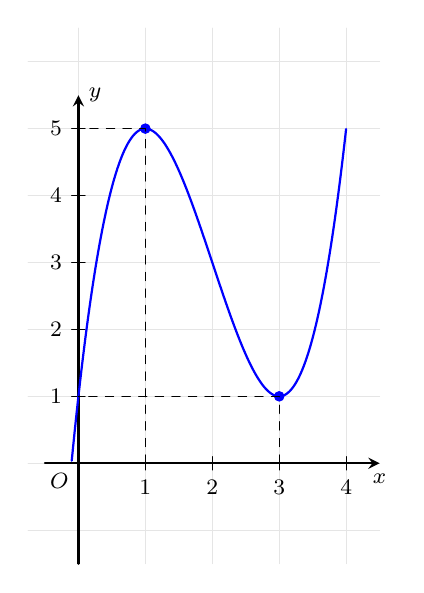
\begin{tikzpicture}[scale=.85, font=\footnotesize, line join=round, line cap=round, >=stealth]
			% Lưới nền
			\draw[gray!20, thin] (-0.75,-1.5) grid (4.5,6.5);
			
			% Trục tọa độ
			\draw[-stealth, thick] (-0.5,0) -- (4.5,0) node[below] {$x$};
			\draw[-stealth, thick] (0,-1.5) -- (0,5.5) node[right] {$y$};
			
			% Gốc tọa độ
			\node at (0,0) [below left] {$O$};
			
			% Đánh dấu trục
			\foreach \x in {1,2,3,4}
			\draw (\x,0.1) -- (\x,-0.1) node[below] {$\x$};
			\foreach \y in {1,2,3,4,5}
			\draw (0.1,\y) -- (-0.1,\y) node[left] {$\y$};
			% Vẽ đồ thị hàm số y = x^3 - 6x^2 + 9x + 1
			\draw[blue, thick, domain=-0.1:4, samples=200] 
			plot (\x, {(\x)^3 - 6*(\x)^2 + 9*(\x) + 1});
			% Đánh dấu điểm cực trị
			\filldraw[blue] (1,5) circle (2pt) ;
			\filldraw[blue] (3,1) circle (2pt);
			
			% Đường hỗ trợ minh họa cực trị
			\draw[dashed] (1,0) |- (0,5);
			\draw[dashed] (3,0) |- (0,1);
	\end{tikzpicture}}
	\loigiai{
		\begin{itemchoice}
			\itemch Dựa và đồ thị, hàm số có $2$ điểm cực trị là $x=1$ và $x=3$.
			\itemch Hàm số đồng biến trên khoảng $(-\infty;1)$, $(3;+\infty)$ và nghịch biến trên khoảng $(1;3)$.
			\itemch Ta có $\lim\limits_{x\to +\infty} y=+\infty$ nên hàm số không có giá trị lớn nhất của hàm số trên khoảng $(0;+\infty)$.
			\itemch Ta có $f(1)=a+b+c+d$, dựa cò đồ thị $f(1)=5$. Suy ra $a + b + c + d = 5$.
		\end{itemchoice}
	}
\end{ex}
\begin{ex}%%[Dự án đề kiểm tra Toán 12 GHKI NH25-26- Nguyễn Văn Sang ]%[THPT NGUYỄN BỈNH KHIÊM - Hà Nội]%[2D1V3-6]
	Số lượng sản phẩm bán được của một công ty trong $x$ (tháng) được tính theo công thức $S(x) = 200 \left(5 - \dfrac{9}{x + 2}\right)$, trong đó $x \geq 1$. Khi đó $S'(x)$ biểu thị tốc độ thay đổi của số lượng sản phẩm bán được theo thời gian.
	\choiceTF
	{\True Công ty bán được $775$ sản phẩm trong $6$ tháng}
	{\True Đạo hàm $S'(x) = \dfrac{1800}{(x + 2)^2}$}
	{Nếu công ty duy trì thời gian bán hàng đủ lâu thì số lượng sản phẩm bán được sẽ vượt mức $1000$}
	{\True Doanh số của công ty tăng trưởng chậm dần theo thời gian}
	\loigiai{
		\begin{itemchoice}
			\itemch \textbf{Tính số sản phẩm sau $6$ tháng}
			$$
			S(6) = 200\left(5 - \dfrac{9}{6 + 2}\right) = 200\left(5 - \dfrac{9}{8}\right) = 200 \times \dfrac{31}{8} = 775.
			$$
			\itemch \textbf{Tính đạo hàm}
			$$
			S(x) = 1000 - \dfrac{1800}{x + 2} \quad \Rightarrow \quad S'(x) = \dfrac{1800}{(x + 2)^2}.
			$$
			\itemch \textbf{Xét giới hạn khi $x \to +\infty$}
			$$
			\lim_{x \to +\infty} S(x) = \lim_{x \to +\infty} 200\left(5 - \dfrac{9}{x + 2}\right) = 1000.
			$$
			Hàm $S(x)$ tiến tới $1000$ nhưng \textbf{không bao giờ vượt quá} $1000$.
			\itemch \textbf{Xét tốc độ tăng trưởng}
			$$
			S'(x) = \dfrac{1800}{(x + 2)^2}.
			$$
			Vì $(x + 2)^2$ tăng khi $x$ tăng $\Rightarrow S'(x)$ giảm $\Rightarrow$ tốc độ tăng trưởng chậm dần.
		\end{itemchoice}
	}
\end{ex}
\begin{ex}%%[Dự án đề kiểm tra Toán 12 GHKI NH25-26- Nguyễn Văn Sang ]%[THPT NGUYỄN BỈNH KHIÊM - Hà Nội]%[2D1H5-7]
	Cho hàm số $y = \dfrac{x^2 + x + 7}{x + 2}$.
	\choiceTF
	{Hàm số đã cho có đạo hàm là $y' = \dfrac{x^2 + 4x - 5}{x + 2}$}
	{\True Điểm $A(-5; -9)$, $B(1; 3)$ lần lượt là điểm cực đại và điểm cực tiểu của đồ thị hàm số trên}
	{\True Đường tiệm cận xiên của đồ thị hàm số đã cho là $y = x - 1$}
	{Đồ thị hàm số đã cho đi qua $12$ điểm có hoành độ và tung độ là những số nguyên}
	\loigiai{
		\begin{itemchoice}
			\itemch \textbf{Kiểm tra đạo hàm}
			$$
			y' = \dfrac{(2x + 1)(x + 2) - (x^2 + x + 7)}{(x + 2)^2} = \dfrac{x^2 + 4x - 5}{(x + 2)^2}.
			$$
			\itemch \textbf{Xác định điểm cực trị}\\
			Giải phương trình $y' = 0 \Leftrightarrow x^2 + 4x - 5 = 0 \Leftrightarrow \hoac{&x=-5\\&x=1.}$\\
			Bảng biến thiên
			\begin{center}
				
\begin{tikzpicture}[scale=1, font=\footnotesize, line join=round, line cap=round, >=stealth]
					\tkzTabInit[nocadre=false,lgt=1,espcl=2,deltacl=0.5]
					{$x$/1, $f'(x)$/1, $f(x)$/2}
					{$-\infty$, $-5$, $-2$, $1$, $+\infty$}
					\tkzTabLine{, + ,  0 ,  - ,  d ,  - ,  0 ,  + ,}
					\tkzTabVar{-/$-\infty$ , +/$-9$ , -D+/$-\infty$/$+\infty$ , -/$3$ , +/$+\infty$}
				\end{tikzpicture}
			\end{center}
			Dựa vào bảng biến thiên, ta có điểm $A(-5; -9)$, $B(1; 3)$ lần lượt là điểm cực đại và điểm cực tiểu của đồ thị hàm số.
			\itemch \textbf{Tìm tiệm cận xiên}
			$$
			y = \dfrac{x^2 + x + 7}{x + 2} = (x - 1) + \dfrac{9}{x + 2}.
			$$
			Suy ra tiệm cận xiên $y = x - 1$.
			\itemch \textbf{Đếm điểm nguyên:}\\
			Điều kiện: $x + 2$ phải là ước của $9$ (vì $y = x - 1 + \dfrac{9}{x + 2}$).\\
			Các ước $\pm 1, \pm 3, \pm 9$ $\Rightarrow$ $6$ giá trị $x$: 
			$x = -11, -5, -3, -1, 1, 7$.\\
			Tương ứng $6$ điểm nguyên: 
			$(-11; -13)$, $(-5; -9)$, $(-3; -13)$, $(-1; 7)$, $(1; 3)$, $(7; 7)$.\\
			Suy ra chỉ có $6$ điểm có toạ độ nguyên.
		\end{itemchoice}
	}
\end{ex}
\begin{ex}%%[Dự án đề kiểm tra Toán 12 GHKI NH25-26- Nguyễn Văn Sang ]%[THPT NGUYỄN BỈNH KHIÊM - Hà Nội]%[2D1V3-6]
	Một doanh nghiệp sản xuất và tiêu thụ một loại sản phẩm. Trong một ngày, nếu doanh nghiệp sản xuất và tiêu thụ $x$ sản phẩm ($x \in \mathbb{N}$, $1 \leq x \leq 186$) thì chi phí trung bình cho mỗi sản phẩm là
	$$
	\overline{C}(x) = x^2 - 6x + 140 + \dfrac{750}{x} \ (\text{USD/sản phẩm}.)
	$$
	và toàn bộ chúng được bán với giá $(1400 - 7{,}5x)$ (USD) một sản phẩm. Giả sử toàn bộ $x$ sản phẩm sản xuất ra đều được tiêu thụ hết.
	\choiceTF
	{\True Số tiền doanh nghiệp thu được là $F(x) = 1400x - 7{,}5x^2$ (USD)}
	{\True Chi phí doanh nghiệp phải bỏ ra là $C(x) = x^3 - 6x^2 + 140x + 750$ (USD)}
	{\True Lợi nhuận doanh nghiệp thu được là $P(x) = -x^3 - 1,5x^2 + 1260x - 750$ (USD)}
	{\True Lợi nhuận lớn nhất mà doanh nghiệp thu được là $15\,850$ (USD)}
	\loigiai{
		\begin{itemchoice}
			\itemch \textbf{Kiểm tra doanh thu}
			Doanh thu = Giá bán $\times$ Số lượng
			$$
			F(x) = (1400 - 7{,}5x) \cdot x = 1400x - 7{,}5x^2.
			$$
			\itemch \textbf{Kiểm tra chi phí}\\
			Chi phí = Chi phí trung bình $\times$ Số lượng
			$$
			C(x) = \overline{C}(x) \cdot x = \left(x^2 - 6x + 140 + \dfrac{750}{x}\right) \cdot x = x^3 - 6x^2 + 140x + 750.
			$$
			\itemch \textbf{Kiểm tra lợi nhuận}\\
			Lợi nhuận = Doanh thu - Chi phí
			$$
			P(x) = F(x) - C(x) = (1400x - 7{,}5x^2) - (x^3 - 6x^2 + 140x + 750).
			$$
			$$
			= -x^3 - 1{,}5x^2 + 1260x - 750.
			$$
			\itemch \textbf{Tính lợi nhuận lớn nhất}\\
			Đạo hàm $P'(x) = -3x^2 - 3x + 1260$.\\
			Giải phương trình: $-3x^2 - 3x + 1260 = 0 \Leftrightarrow \hoac{&x=20 &\text{(nhận)}\\&x=-21 &\text{(loại).}}$\\
			Tính giá trị tại $x = 20$ ta có
			$$
			P(20) = -(20)^3 - 1,5(20)^2 + 1260(20) - 750 = 15\,850.
			$$
		\end{itemchoice}
	}
\end{ex}
\TNSA

%\caukq
%%%=============BT_1=============%%%
\begin{ex}%[2D1H1-3]%[Lê Hồ Quang Minh - GK1 NguyenBinhKhiem-HN-25-26]
	Cho hàm số $y=\dfrac{mx+2\,025}{x+2}$ với $m$ là tham số. Có bao nhiêu số nguyên dương $m$ để hàm số đã cho nghịch biến trên các khoảng xác định?
	\shortans{$1012$}
	\loigiai{
		Tập xác định của hàm số $\mathscr{D}=\mathbb{R}\setminus\{-2\}$.\\
		Ta có $y'=\dfrac{2m-2\,025}{(x+2)^2}$.\\
		Để hàm số đã cho nghịch biến trên các khoảng xác định, điều kiện là
		$$y'<0,\forall x\ne -2\Leftrightarrow 2m-2025<0\Leftrightarrow m<1012{,}5.$$
		Suy ra, có $1012$ các giá trị nguyên dương của $m$ thỏa mãn yêu cầu bài toán.
	}
\end{ex}
%%%=============================%%%

%%%=============BT_2=============%%%
\begin{ex}%[2D1V3-2]%[Lê Hồ Quang Minh - GK1 NguyenBinhKhiem-HN-25-26]
	\immini[thm]{Cho hình vuông $ABCD$ có cạnh bằng $1$ và cung $\stackrel\frown{BD}$ là một phần tư đường tròn tâm $A$, bán kính $AB$ (tham khảo hình vẽ bên). Gọi $M$ là một điểm di động trên cung $\stackrel\frown{BD}$. Tiếp tuyến với cung $\stackrel\frown{BD}$ tại điểm $M$ cắt cạnh $CD$ tại điểm $P$ và cắt cạnh $BC$ tại điểm $Q$. Tính độ dài đoạn thẳng $DP$ để $PQ$ có độ dài nhỏ nhất (\textit{làm tròn kết quả đến hàng phần trăm}).}
	{\begin{tikzpicture}[line join = round, line cap=round,>=stealth,font=\footnotesize,scale=1]
			\def\s{4}
			\path
			(0:0) coordinate (A)
			(0:\s) coordinate (B)
			(-90:\s)coordinate (D)
			($(B)+(D)-(A)$) coordinate (C)
			(-60:\s) coordinate (M)
			($(M)!0.5!90:(A)$) coordinate (E)
			(intersection of M--E and B--C) coordinate (Q)
			(intersection of M--E and D--C) coordinate (P);
			\draw (A) -- (B) -- (C) -- (D) -- cycle
			(A)--(M) (P)--(Q);
			\draw (D) arc (-90:0:\s);
			\pic[draw,angle radius=5]{right angle=A--M--Q};
			\foreach \p/\r in {A/150, B/30,C/-30,D/-150,M/-60,P/-90,Q/0}
			\fill (\p) circle (1pt) node[shift={(\r:3mm)}]{$\p$};
	\end{tikzpicture}}
	\shortans{$0{,}41$}
	\loigiai{
		\immini[thm]{
			Đặt $\alpha=\widehat{DAP}=\widehat{MAP}$, $\beta=\widehat{BAQ}=\widehat{MAQ}$. Ta có $\alpha+\beta=45^\circ$.\\
			Ta có
			\begin{eqnarray*}
				PQ&=&PM+QM=DP+BQ \\
				&=&AD\tan\alpha+AB\tan\beta=\tan\alpha+\tan\beta \\
				&=&\tan\alpha+\tan(45^\circ-\alpha)=\tan\alpha+\dfrac{1-\tan\alpha}{1+\tan\alpha}\\
				&=&\dfrac{x^2+1}{x+1}.
			\end{eqnarray*}
		}
		{\begin{tikzpicture}[line join = round, line cap=round,>=stealth,font=\footnotesize,scale=1]
				\def\s{4}
				\path
				(0:0) coordinate (A)
				(0:\s) coordinate (B)
				(-90:\s)coordinate (D)
				($(B)+(D)-(A)$) coordinate (C)
				(-60:\s) coordinate (M)
				($(M)!0.5!90:(A)$) coordinate (E)
				(intersection of M--E and B--C) coordinate (Q)
				(intersection of M--E and D--C) coordinate (P);
				\draw (A) -- (B) -- (C) -- (D) -- cycle
				(A)--(M) (P)--(Q) (A)--(P) (A)--(Q);
				\draw (D) arc (-90:0:\s);
				\pic[draw,angle radius=5]{right angle=A--M--Q};
				\pic[draw,angle radius=5]{right angle=A--B--Q};
				\pic[draw,angle radius=5]{right angle=A--D--P};
				\pic[draw,angle radius=15]{angle=P--A--M};
				\pic[draw,angle radius=17]{angle=M--A--Q};
				\foreach \p/\r in {A/150, B/30,C/-30,D/-150,M/-60,P/-90,Q/0}
				\fill (\p) circle (1pt) node[shift={(\r:3mm)}]{$\p$};
				\path
				(-70:1.2) node[scale=1]{$\alpha$}
				(-40:1.2) node[scale=1]{$\beta$};
		\end{tikzpicture}}
		Với $x=\tan\alpha$ và $x>0$.\\
		Xét hàm số $f(x)=\dfrac{x^2+1}{x+1}$ với $x>0$, ta có $f'(x)=\dfrac{x^2+2x-1}{(x+1)^2}$.\\
		$f'(x)=0\Rightarrow x=-1+\sqrt{2}$.\\
		Ta có bảng biến thiên
		\begin{center}
			
\begin{tikzpicture}
				\tkzTabInit[nocadre=false,lgt=1.2,espcl=3]
				{$x$ /1, $y'$ /1,$y$ /2}
				{$0$,$-1+\sqrt{2}$,$+\infty$}
				\tkzTabLine{,-,0 ,+, }
				\tkzTabVar{+/$1$, -/$2\sqrt{2}-2$ ,+/$+\infty$}
			\end{tikzpicture}
		\end{center}
		Vậy, để $PQ$ có độ dài nhỏ nhất thì $x=\tan\alpha=-1+\sqrt{2}$. Khi đó $DP=AD\tan\alpha=1\cdot \left(-1+\sqrt{2}\right)\approx 0{,}41$.
	}
\end{ex}
%%%=============================%%%

%%%=============BT_3=============%%%
\begin{ex}%[2D1V4-3]%[Lê Hồ Quang Minh - GK1 NguyenBinhKhiem-HN-25-26]
	Biết rằng hai đường tiệm cận của đồ thị hàm số $y = -2x + 1 + \dfrac{2}{x-2}$ tạo với nhau một góc $\alpha$, hãy tính $\tan \alpha$ (viết kết quả ở dạng số thập phân).
	\shortans{0,5}
	\loigiai{
		Tập xác định $\mathscr{D} = \mathbb{R} \setminus \{2\}$.\\
		Ta có $\lim\limits_{x \to 2^+} y = \lim\limits_{x \to 2^+} \left(-2x + 1 + \dfrac{2}{x-2}\right) = +\infty$ và $\lim\limits_{x \to 2^-} y = \lim\limits_{x \to 2^-} \left(-2x + 1 + \dfrac{2}{x-2}\right) = -\infty$.\\
		Suy ra đồ thị hàm số có tiệm cận đứng là $d_1\colon x = 2$ (hay $x - 2 = 0$).\\
		Lại có $\lim\limits_{x \to\pm \infty} \left[y - (-2x+1)\right] = \lim\limits_{x \to\pm \infty} \dfrac{2}{x-2} = 0$.\\
		Suy ra đồ thị hàm số có tiệm cận xiên là $d_2\colon y = -2x + 1$ (hay $2x + y - 1 = 0$).\\
		Đường thẳng $d_1$ có vectơ pháp tuyến là $\vec{n}_1 = (1; 0)$.\\
		Đường thẳng $d_2$ có vectơ pháp tuyến là $\vec{n}_2 = (2; 1)$.\\
		Gọi $\alpha$ là góc giữa hai đường tiệm cận $d_1$ và $d_2$, ta có:
		$$ \cos \alpha = \dfrac{|\vec{n}_1 \cdot \vec{n}_2|}{|\vec{n}_1| \cdot |\vec{n}_2|} = \dfrac{|1 \cdot 2 + 0 \cdot 1|}{\sqrt{1^2 + 0^2} \cdot \sqrt{2^2 + 1^2}} = \dfrac{2}{\sqrt{1} \cdot \sqrt{5}} = \dfrac{2}{\sqrt{5}}. $$
		Ta có $1 + \tan^2 \alpha = \dfrac{1}{\cos^2 \alpha} \Rightarrow \tan^2 \alpha = \dfrac{1}{\cos^2 \alpha} - 1 = \dfrac{1}{\left(\dfrac{2}{\sqrt{5}}\right)^2} - 1 = \dfrac{5}{4} - 1 = \dfrac{1}{4}$.\\
		Vì $0^\circ \le \alpha \le 90^\circ$ nên $\tan \alpha \ge 0$, do đó $\tan \alpha = \sqrt{\dfrac{1}{4}} = \dfrac{1}{2} = 0{,}5$.
	}
\end{ex}
%%%=============================%%%

%%%=============BT_4=============%%%
\begin{ex}%[2D1V4-3]%[Lê Hồ Quang Minh - GK1 NguyenBinhKhiem-HN-25-26]
	Đồ thị hàm số $y = x^3 - 6x^2 + 2$ có hai điểm cực trị $A$ và $B$ cùng với gốc tọa độ $O$ tạo thành một tam giác có diện tích bằng bao nhiêu?
	\shortans{4}
	\loigiai{
		Tập xác định $D=\mathbb{R}$.\\
		Ta có $y' = 3x^2 - 12x$.\\
		Ta có $y' = 0 \Leftrightarrow 3x^2 - 12x = 0 \Leftrightarrow \hoac{&x=0\\&x=4.}$\\
		Ta có $y(0)=2$, $y(4)=-30$.\\
		Suy ra hai điểm cực trị là $A(0; 2)$ và $B(4; -30)$.\\
		Ta có $OA = \sqrt{(0-0)^2 + (2-0)^2} = 2$.\\
		Ta thấy hai điểm $O(0; 0)$ và $A(0; 2)$ cùng nằm trên trục $Oy$.\\
		Do đó chiều cao $h$ của tam giác $OAB$ ứng với cạnh $OA$ là khoảng cách từ $B$ đến trục $Oy$.\\
		Suy ra $h = \mathrm d(B, Oy) = |x_B| = |4| = 4$.\\
		Vậy diện tích tam giác $OAB$ là $S_{\triangle OAB} = \dfrac{1}{2} \cdot OA \cdot h = \dfrac{1}{2} \cdot 2 \cdot 4 = 4$.
	}
\end{ex}
%%%=============================%%%

%%%=============BT_5=============%%%
\begin{ex}%[2D1V3-6]%[Lê Hồ Quang Minh - GK1 NguyenBinhKhiem-HN-25-26]
	\immini[thm]{Một ngọn hải đăng đặt tại vị trí $A$ cách bờ biển một khoảng $AB=5$ km. Trên bờ biển có một cái kho ở vị trí $C$ cách $B$ một khoảng bằng $7$ km. Người canh hải đăng có thể chèo thuyền từ $A$ đến điểm $M$ trên bờ biển với vận tốc $4$ km/h rồi đi bộ thẳng đến $C$ với vận tốc $6$ km/h. Xác định khoảng cách từ điểm $M$ đến điểm $B$ để người đó đến kho nhanh nhất (làm tròn kết quả đến hàng phần trăm).
	}{\begin{tikzpicture}[line join = round, line cap=round,>=stealth,font=\footnotesize,scale=0.6]
			\coordinate (B) at (0,0);
			\coordinate (A) at (0,5);
			\coordinate (C) at (7,0);
			\coordinate (M) at (3.5,0);
			\draw (A) -- (B) -- (C);
			\draw (A) -- (M);
			\draw (0.2,0) -- (0.2,0.2) -- (0,0.2);
			\node[left] at (A) {$A$};
			\node[below] at (B) {$B$};
			\node[below] at (C) {$C$};
			\node[below] at (M) {$M$};
			\node[left] at (0,2.5) {$5$ km};
			\draw[<->] (0,-0.7) -- (7,-0.7);
			\node[below] at (3.5,-0.9) {$7$ km};
		\end{tikzpicture}}
	\shortans{4,47}
	\loigiai{
		Đặt $BM=x$ (km), điều kiện $0\le x\le 7$.
		Khi đó, $MC=BC-BM=7-x$ (km).\\
		Trong tam giác vuông $ABM$, ta có $AM=\sqrt{AB^2+BM^2}=\sqrt{5^2+x^2}=\sqrt{25+x^2}$ (km).\\
		Thời gian người đó chèo thuyền từ $A$ đến $M$ là $t_1=\dfrac{AM}{4}=\dfrac{\sqrt{25+x^2}}{4}$ (giờ).\\
		Thời gian người đó đi bộ từ $M$ đến $C$ là $t_2=\dfrac{MC}{6}=\dfrac{7-x}{6}$ (giờ).\\
		Tổng thời gian để người đó di chuyển từ $A$ đến $C$ là
		$$T(x)=t_1+t_2=\dfrac{\sqrt{25+x^2}}{4}+\dfrac{7-x}{6}.$$
		Bài toán trở thành tìm giá trị nhỏ nhất của hàm số $T(x)$ trên đoạn $[0;7]$.
		Ta có đạo hàm
		$$T'(x)=\dfrac{1}{4}\cdot\dfrac{2x}{2\sqrt{25+x^2}}-\dfrac{1}{6}=\dfrac{x}{4\sqrt{25+x^2}}-\dfrac{1}{6}.$$
		Giải phương trình $T'(x)=0$
		\begin{eqnarray*}
			\dfrac{x}{4\sqrt{25 + x^2}} - \dfrac{1}{6} = 0 &\Leftrightarrow& \dfrac{x}{4\sqrt{25 + x^2}} = \dfrac{1}{6} \\
			&\Leftrightarrow& 6x = 4\sqrt{25 + x^2} \\
			&\Leftrightarrow& 3x = 2\sqrt{25 + x^2} \\
			&\Leftrightarrow&\heva{&x \ge 0 \\&9x^2 = 4(25 + x^2)} \\
			&\Leftrightarrow& \heva{&x \ge 0 \\ &9x^2 = 100 + 4x^2} \\
			&\Leftrightarrow&\heva{&x \ge 0 \\ &5x^2 = 100} \\
			&\Leftrightarrow& x^2 = 20 \Leftrightarrow x = 2\sqrt{5} \quad (\text{vì } x \ge 0).
		\end{eqnarray*}
		Ta có $x=2\sqrt{5}\approx 4{,}47\in[0;7]$.
		Lập bảng biến thiên của hàm số $T(x)$ trên đoạn $[0;7]$, ta có
		\begin{center}
			
\begin{tikzpicture}[line join=round, line cap=round, >=stealth, scale=1]
				\tkzTabInit[nocadre=false, lgt=1.2, espcl=3, deltacl=0.5]
				{$x$/1, $T'(x)$/1, $T(x)$/3}
				{ $0$, $2\sqrt{5}$, $7$}
				\tkzTabLine{, -, 0, +, }
				\tkzTabVar{+/$\dfrac{29}{12}$,-/$\dfrac{14+5\sqrt{5}
					}{12}$, +/$\dfrac{\sqrt{74}}{4}$}
			\end{tikzpicture}
		\end{center}
		Vậy để đến kho nhanh nhất thì người đó cần đến điểm $M$ trên bờ biển cách $B$ một khoảng là $2\sqrt{5}\approx 4{,}47$ km.
	}
\end{ex}
%%%=============================%%%

%%%=============BT_6=============%%%
\begin{ex}%[2D1V3-6]%[Lê Hồ Quang Minh - GK1 NguyenBinhKhiem-HN-25-26]
	Một bồn chứa dầu được thiết kế với hai đầu là hai nửa hình cầu có bán kính $r$ (m) và phần thân ở giữa là một hình trụ có bán kính đáy $r$ (m) và chiều cao $h$ (m) (tham khảo hình vẽ dưới đây). Toàn bộ bồn chứa được yêu cầu có thể tích là $9\pi$ (m$^3$) và để đảm bảo tính ổn định trong quá trình vận chuyển, chiều cao $h$ của phần hình trụ phải thỏa mãn điều kiện $h\ge 2$ (m). Chi phí để làm bồn phụ thuộc vào diện tích toàn bộ bề mặt ngoài của bồn (bao gồm mặt xung quanh của phần hình trụ và bề mặt của hai nửa hình cầu). Hãy xác định bán kính $r$ (m) để chi phí làm bồn là nhỏ nhất (viết kết quả ở dạng số thập phân).
	\begin{center}
		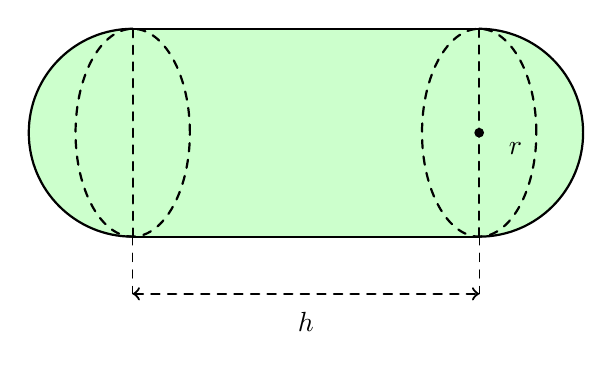
\begin{tikzpicture}[line join=round, line cap=round, scale=1.1]
			% --- tham số ---
			\def\H{4.0}        % chiều dài phần trụ (h)
			\def\R{1.2}        % bán kính (r)
			\pgfmathsetmacro{\XR}{0.55*\R}  % bán trục elip theo phương x để tạo phối cảnh
			
			% --- thân bồn: trụ + hai bán cầu (tô nền và viền) ---
			\fill[green!20]
			(-\H/2,-\R) -- (\H/2,-\R)
			arc[start angle=-90,end angle=90,radius=\R] --
			(-\H/2,\R)
			arc[start angle=90,end angle=270,radius=\R] -- cycle;
			
			% viền trên, dưới, và hai bán cầu
			\draw[thick] (-\H/2,\R) -- (\H/2,\R);
			\draw[thick] (-\H/2,-\R) -- (\H/2,-\R);
			\draw[thick] (\H/2,-\R) arc[start angle=-90,end angle=90,radius=\R];
			\draw[thick] (-\H/2,\R)  arc[start angle=90, end angle=270,radius=\R];
			
			% --- elip 3D và trục ở hai đầu ---
			% trục giữa hai bán cầu (nét đứt)
			\draw[dashed,thick] (-\H/2,-\R) -- (-\H/2,\R);
			\draw[dashed,thick] (\H/2,\R) -- (\H/2,-\R);   % giống mẫu: có mũi tên đi xuống
			
			% elip (đường sinh ẩn) – đặt đúng tâm ở hai đầu
			\draw[dashed,thick] (-\H/2,0) ellipse [x radius=\XR, y radius=\R];
			\draw[dashed,thick] ( \H/2,0) ellipse [x radius=\XR, y radius=\R];
			
			% --- chữ và kích thước ---
			% \node at (0,0) {Oil tank}};
			
			% kích thước h (mũi tên hai đầu, có đường dóng)
			\draw[dashed] (-\H/2,-\R) -- (-\H/2,-1.55*\R);
			\draw[dashed] ( \H/2,-\R) -- ( \H/2,-1.55*\R);
			\draw[<->, dashed, thick] (-\H/2,-1.55*\R) -- (\H/2,-1.55*\R)
			node[midway,below=3pt] {$h$};
			
			% bán kính r: chấm tâm + nhãn bên phải
			\fill ( \H/2,0) circle (1.6pt);
			\node[anchor=north] at (\H/2+0.35*\R,0) {$r$};
		\end{tikzpicture}
	\end{center}
	\shortans{1,5}
	\loigiai{
		Thể tích của bồn chứa dầu gồm thể tích của một hình trụ có bán kính đáy $r$, chiều cao $h$ và thể tích của một hình cầu có bán kính $r$.
		Theo giả thiết, thể tích của bồn là $9\pi$ (m$^3$), ta có phương trình
		$$V=\pi r^2h+\dfrac{4}{3}\pi r^3=9\pi\Leftrightarrow r^2h+\dfrac{4}{3}r^3=9\Leftrightarrow h=\dfrac{9}{r^2}-\dfrac{4}{3}r.$$
		Điều kiện $h\ge 2$ tương đương với $\dfrac{9}{r^2}-\dfrac{4}{3}r\ge 2$.
		Vì $r>0$, ta nhân hai vế của bất phương trình với $3r^2$, ta được
		$$27-4r^3\ge 6r^2\Leftrightarrow 4r^3+6r^2-27\le 0.$$
		Xét hàm số $f(r)=4r^3+6r^2-27$ với $r>0$.\\
		Ta có $f'(r)=12r^2+12r>0,\forall r>0$.\\
		Do đó, hàm số $f(r)$ đồng biến trên $(0;+\infty)$.\\
		Mặt khác, $f\left(\dfrac{3}{2}\right)=4\cdot\left(\dfrac{3}{2}\right)^3+6\cdot\left(\dfrac{3}{2}\right)^2-27=0$.
		Từ đó suy ra $4r^3+6r^2-27\le 0\Leftrightarrow 0<r\le\dfrac{3}{2}$.\\
		Chi phí làm bồn chứa phụ thuộc vào diện tích bề mặt ngoài của bồn. Diện tích này bằng tổng diện tích xung quanh của hình trụ và diện tích mặt cầu.
		$$S(r)=2\pi r h+4\pi r^2=2\pi r\left(\dfrac{9}{r^2}-\dfrac{4}{3}r\right)+4\pi r^2=\dfrac{18\pi}{r}-\dfrac{8\pi}{3}r^2+4\pi r^2=\dfrac{18\pi}{r}+\dfrac{4\pi}{3}r^2.$$
		Bài toán trở thành tìm giá trị nhỏ nhất của hàm số $S(r)=\dfrac{18\pi}{r}+\dfrac{4\pi}{3}r^2$ trên nửa khoảng $\left(0;\dfrac{3}{2}\right]$.
		Ta có đạo hàm
		$$S'(r)=-\dfrac{18\pi}{r^2}+\dfrac{8\pi}{3}r=\dfrac{-54\pi+8\pi r^3}{3r^2}.$$
		Với $r\in\left(0;\dfrac{3}{2}\right]$, ta có $r^3\le\left(\dfrac{3}{2}\right)^3=\dfrac{27}{8}$, suy ra $8\pi r^3\le 27\pi<54\pi$.
		Do đó, $S'(r)<0$ với mọi $r\in\left(0;\dfrac{3}{2}\right]$.
		Suy ra hàm số $S(r)$ nghịch biến trên nửa khoảng $\left(0;\dfrac{3}{2}\right]$.
		Do đó, giá trị nhỏ nhất của $S(r)$ đạt được tại $r=\dfrac{3}{2}=1{,}5$.
		
		Vậy để chi phí làm bồn là nhỏ nhất thì bán kính $r=1{,}5$ (m).
	}
\end{ex}
%%%=============================%%%